\documentclass{standalone}

\usepackage[american]{circuitikz}
\usepackage{mathtools}

\begin{document}
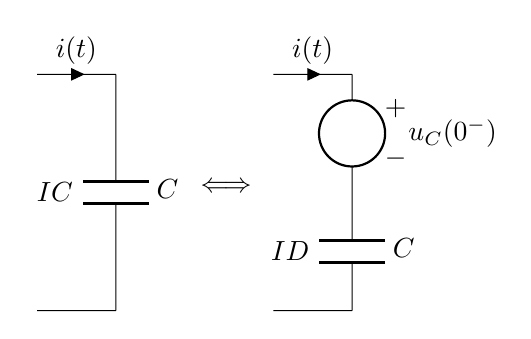
\begin{tikzpicture}
\coordinate(A) at (2.4,-1.75);
  \draw
  (0,0) to [short,-, i=$i(t)$] (1,0)
  (1,0) to [C=$C$,n=C] (1,-3) (C.s) node[left] {$IC$}
  (0,-3) to [short,-] (1,-3)
  (3,0) to [short,-, i=$i(t)$] (4,0)
  (4,-1.5) to [C=$C$,n=C2] (4,-3) (C2.s) node[left] {$ID$}
  (4,0) to [esource, v=$u_C(0^-)$] (4,-1.5)
  (3,0) to [short,-] (4,0)
  (3,-3) to [short,-] (4,-3);
  \node[label=$\Longleftrightarrow$] (A) at ($(A)$) {};
\end{tikzpicture}
\end{document}